\begin{ZhChapter}

\chapter{相關技術與背景}

\section{藍牙低功耗技術}

藍牙技術聯盟(Bluetooth Special Interest Group)在2010年6月發布了可以短距離數據交換和低功耗的藍牙低功耗技術(Bluetooth Low Energy, BLE)。而藍牙低功耗技術被發布後,就被物聯網(IoT)廣泛的應用,包括了家庭娛樂、醫療保健、運動健身、安防以及信標等領域。

藍牙低功耗技術(Bluetooth Low Energy, BLE)是一種功耗極低的技術,這一個技術讓裝置在大部分的時間都在休眠模式,只有在需要使用該裝置時,才會快速喚醒進行工作,這讓BLE裝置僅需要一顆鈕扣電池就可以運作數月甚至數年之久,這讓BLE生產成本更低,且保留了傳統藍牙(Classic Bluetooth)類似的通訊範圍,且一樣相容於手機、平板電腦等設備。

BLE運作在2.4G的ISM頻段,利用FDMA(Frequency Division Multiple Access),將2402MHz至2480MHz分成40個Channel,又將這些Channel又分成兩種傳輸模式,廣播模式(Advertising Mode)及連線模式(Connection-Oriented Mode),其中廣播模式使用了Channel 37、Channel 38、Channel 39,工作頻率分別是2403MHz、2426MHz、2480MHz,剩餘的37個Channel為連接模式使用,如圖\ref{fig: 廣播頻道與資料頻道示意圖}所示。

\begin{figure}[H]
    \centering
    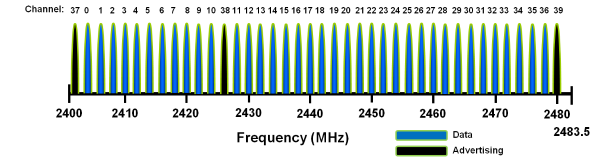
\includegraphics[width = 1\textwidth]{image/ble-phy-channel-assignment.png}
    \caption{廣播頻道與資料頻道示意圖\cite{microchip2023}}
    \label{fig: 廣播頻道與資料頻道示意圖}
\end{figure}

廣播模式和連接模式的運作機制由 BLE 的控制層(Controller Layer)狀態機管理,包括Standby(等待)、Advertising(廣播)、Scanning(掃描)、Initiating(初始化)、Connection(連接)五種狀態 ,如圖\ref{fig: Controller layer 狀態機示意圖}所示。

\begin{figure}[H]
    \centering
    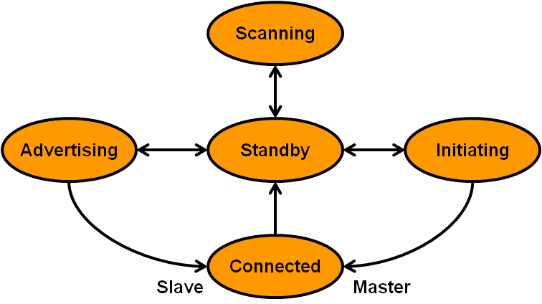
\includegraphics[width = 1\textwidth]{image/ble-link-layer-sm.png}
    \caption{Controller layer 狀態機示意圖\cite{microchip2023}}
    \label{fig: Controller layer 狀態機示意圖}
\end{figure}

\subsection{廣播模式}

在廣播模式 (Advertising Mode)中,會使用Channel 37、Channel 38、channel 39這三個廣播頻道,主要用於掃描裝置、建立通訊頻道和廣播的傳輸,其中廣播者(Advertiser)是由待機狀態(Standby Status)進入廣播狀態(Advertising Status),廣播者會在三個廣播頻道輪流發送廣播封包,讓掃描者(Scanner)可以檢測到其存在,並提供基本的數據,例如:裝置名稱或狀態。

掃描者(Scanner)是由待機狀態(Standby Status)進入掃描狀態(Scanner Status),掃描者會輪流掃描三個廣播頻道的廣播封包,以接收範圍內的所有廣播的資訊,掃描收集數據後,準備與廣播設備建立連接,如圖\ref{fig: 廣播模式示意圖}所示。
\begin{figure}[H]
    \centering
    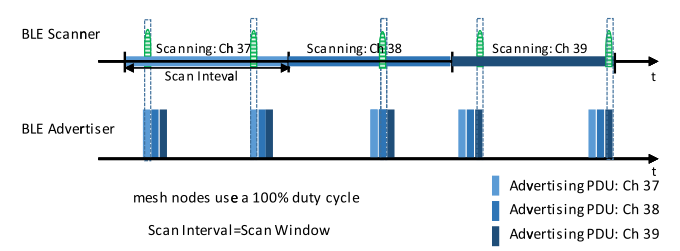
\includegraphics[width = 0.8\textwidth]{image/廣播模式示意圖.png}
    \caption{廣播模式示意圖\cite{9035389}}
    \label{fig: 廣播模式示意圖}
\end{figure}

\subsection{連接模式}

連接模式(Connection-Oriented Mode)中,設備需要首先透過廣播模式建立連接,其中廣播者(Slave)負責發送連線請求的廣播封包,而掃描者(Master)檢測到廣播封包後,從 Standby 進入 Scanning,再進入 Initiating 狀態,開始與廣播設備握手 (Handshake)。

當握手成功後,雙方進入 Connection 狀態。連接建立後,Master 與 Slave 可通過剩餘的 37 個數據頻道進行數據傳輸;Master 負責與多個 Slave 的連線管理,分配專屬的時間槽 (Time Slot) 給各連接設備,即使沒有數據需要傳輸,系統仍會保留固定的時間槽以確保系統的穩定性,避免通訊衝突。圖\ref{fig: 連線模式示意圖}為連線模式示意圖。

\begin{figure}[H]
    \centering
    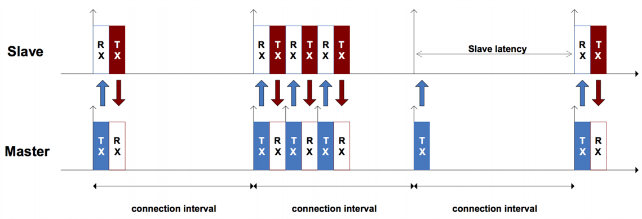
\includegraphics[width = 0.9\textwidth]{image/連線模式示意圖.png}
    \caption{連線模式示意圖\cite{9035389}}
    \label{fig: 連線模式示意圖}
\end{figure}

\subsection{BLE排程機制}

廣播者(Advertiser)和掃描者(Scanner)會在建立連線後,進行數據的交換,當掃描者在三個掃描頻道掃瞄並偵測到廣播者發送的封包後,掃描者會在約 150 微秒($T_{IFS}$)後回應一個 CONNECT\_IND 封包。CONNECT\_IND 封包包含了多項管理連接的參數,例如:影響錨點時間(Anchor Point, AP)的 WinSize 以及 WinOffset。

這些連接參數,Connection Interval (CI)、Anchor Point (AP)和Connection Event (CE)對於裝置之間的排程機制影響非常大,在一個Connection Interval(CI)的時間內,一個Slave裝置只會與Master裝置有一個Connection Event(CE)傳輸時間來進行資料的交換,所以Connection Interval(CI)的時間影響Connection Event(CE)的發生頻率,這直接影響到整個系統的效能及吞吐量,圖\ref{fig: Master 連接建立過程和連接事件}表示了Master連接建立過程和連接事件。  

\begin{figure}[H]
    \centering
    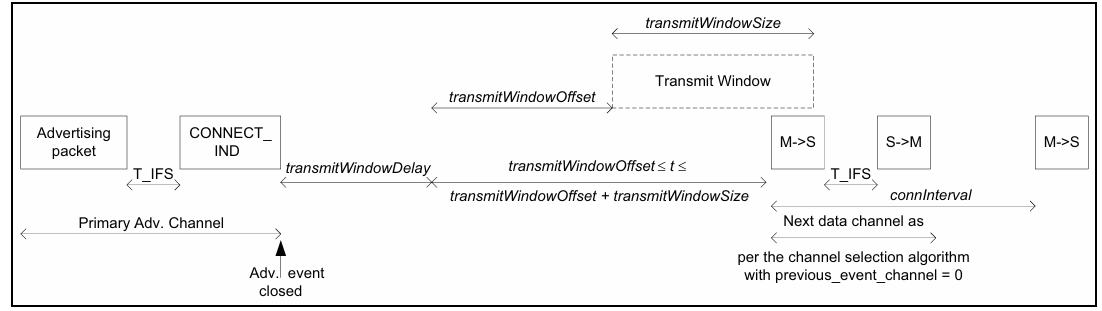
\includegraphics[width = 1\textwidth]{image/Master 連接建立過程和連接事件.png}
    \caption{Master 連接建立過程和連接事件\cite{bluetooth2016core}}
    \label{fig: Master 連接建立過程和連接事件}
\end{figure}

錨點(Anchor Point, AP)是 BLE 連線中用來做為 Master 與 Slave 雙方傳輸時間的參考點,確保雙方能在預期的時刻進行資料交換。透過錨點的設置,Slave 可以準確地進入低功耗睡眠與喚醒,達到節能與通訊準確的目的。

CONNECT\_IND封包會在 $t_{ind}$ 時間內完成傳輸,Master 會在\ref{eq: a}式至\ref{eq: b}式的時間內設置第一個錨點(Anchor Point, AP),其中 transmitWindowDelay 通常為 $1.25\,{ms}$,用來同步 Master 與 Slave。

transmitWinOffset 與 transmitWinSize 分別由\ref{eq: c}式與\ref{eq: d}式算出。WinOffset代表錨點(Anchor Point, AP)的偏移量;WinSize代表錨點(Anchor Point, AP)可能發生的時間範圍\cite{10.1145/3412382.3458271}。

\begin{equation}
t_{ind} + transmitWindowDelay + transmitWinOffset
\label{eq: a}
\end{equation}

\begin{equation}
t_{ind} + transmitWindowDelay + transmitWinOffset + transmitWinSize
\label{eq: b}
\end{equation}

\begin{equation}
transmitWinOffset = WinOffset \times 1.25\, ms
\label{eq: c}
\end{equation}

\begin{equation}
transmitWinSize = WinSize \times 1.25\, ms 
\label{eq: d}
\end{equation}

\section{藍牙網狀網路}

藍牙網狀網路(Bluetooth Mesh)是由藍牙技術聯盟(Bluetooth Special Interest Group)於2017年發布的標準,旨在解決傳統藍牙技術在物聯網(IoT)應用中的傳輸距離限制。藍牙網狀網路允許多個BLE裝置之間建立一個可靠且可擴展的網狀結構,這使得裝置之間可以進行多跳傳輸,從而擴大了傳輸距離和覆蓋範圍。

Bluetooth Mesh 是基於藍牙低功耗(Bluetooth Low Energy, BLE)的網狀網路技術,是多個裝置進行多對多(many-to-many)連接的拓樸技術,可以將資料從BLE Mesh中的其中一個節點,發送至BLE Mesh中的任何一個節點,且任兩個節點間的傳輸路徑,並不會只有一條,因為這種多重路徑(multi-path)的特性,讓Mesh中如果有一個節點故障,也不會因此癱瘓整個系統。此技術有效解決了 BLE 在長距離和多設備連接上的限制,擴展了 BLE 的應用範圍,特別適用於無線感測網路(Wireless Sensor Networks, WSN)和物聯網(IoT)環境。

Bluetooth Mesh 保有BLE的優點,並改善BLE傳輸範圍有限的問題,Bluetooth Mesh的網路架構分為 Flooding 模式及Routing 模式,Flooding Mesh 是大多數 BLE Mesh 協定採用的傳輸模式,利用廣播方式傳送訊息,無需建立節點間的連接,節點將訊息以廣播模式傳遞給通訊範圍內的所有節點,節點收到訊息後再次廣播,直到訊息傳遞至目標節點為止。

Routing Mesh 使用連接模式,節點需在訊息傳輸前建立節點間的連接,確保訊息傳遞有序且可靠。節點之間先建立連接,資料通過預設路徑逐步傳遞至目的節點,並根據需求動態調整路由,因為資料傳輸通過固定路徑,減少碰撞和干擾,讓傳輸更穩定。也因為訊息傳遞通過固定的路徑,降低重複廣播次數,節省了不必要的電能消耗。Routing Mesh 資料傳輸的方式確保資料完整傳遞,即使網路繁忙也能正常運作。相對的缺點也顯而易見,因為資料傳遞時,節點間需建立連接,設計上比較複雜而增加實現難度。且建立連接需耗費額外時間,當路徑上的節點完成所有連接後才會開始傳輸,所以網路啟動比較慢。也會因為接點間連接路徑較長,讓資料傳遞時間增加,最後產生較高的傳輸延遲。

\section{分時多工與BLE中的CI與CE機制}

分時多工 (Time Division Multiple Access, TDMA) 如字面上的意義,它一種將時間分割的通訊技術,讓多個裝置可以高效的共享同一傳輸介質進行傳輸。TDMA 將時間劃分為多個時槽 (Time Slots),每個裝置只能在指定的時槽內進行傳輸,這確保了同一時刻,只有一個裝置進行傳輸,其他的裝置在同一個時間下(相同Time slot),都處於等待的狀態,可以確保訊號穩定且不重疊,有效避免了訊號重疊和干擾而導致的數據丟失。

在BLE中,TDMA的理念被具體實現在連線模式下的CI與CE設計中。BLE通訊雙方在建立連線後,會協商出一個固定的CI,作為接下來通訊週期的基本單位。每個CI之內,雙方僅在特定的CE中進行資料交換,其餘時間則處於睡眠或非活躍狀態。

這樣的設計與TDMA的概念密切相關:每個BLE連線設備實際上都在預定的時槽(即CE時間內)進行資料交換,彼此間在時間上分離,以避免干擾與資源衝突。尤其在多裝置共存環境中,例如一個主裝置(Central)與多個從裝置(Peripheral)連線時,主裝置會根據各連線的CI設計,輪流與不同的裝置進行資料交換,實現一種類似TDMA的排程與存取控制機制。

\section{目的地傾向傳輸}

FruityMesh是一個專門為BLE Mesh Network所開發的開源連接模式之網路協定,在 FruityMesh 的傳輸機制中,訊息從一個節點發送至中繼節點時,中繼節點會廣播訊息給所有相鄰節點,相鄰的節點又會在廣播給其相鄰的節點,直到目標節點,而廣播風暴會造成節點間多餘不必要的資料傳輸,而增加網路的負擔。為了解決廣播風暴問題,目的地傾向傳輸(Destination-Oriented Transmission, DOT)\cite{112TIT00392032}機制,通過引入方向性和目的傾向的傳輸策略,優化封包的傳輸過程,減少網路負載與封包重傳,提升傳輸效率與穩定性。

DOT 機制利用樹狀架構中的 Level 層級概念,在假設封包都是以根(Root)節點為目的端的前提下,為每個節點計算其所屬層級,使用 FIND\_LEVEL 封包進行層級標記,而根節點的Level值最低,傳輸方向封包只需傳遞至 Level 較低 的節點,避免無意義的廣播。DOT 在中繼節點限制封包的傳輸方向,僅向 Level 較低的節點傳輸封包,這種方式有效減少了網路流量,降低碰撞率,並提升了傳輸可靠性。

\section{目的地傾向切換傳輸}

目的地傾向切換傳輸(Destination Oriented Switch Transmission, DOST)\cite{112TIT00392032}機制進一步解決角色身份重疊與傳輸重疊的問題,通過啟用與禁用連線的方式,降低網路負載並避免封包重傳,解決BLE網狀網路節點可能因同時扮演Master和Slave角色衝突而導致的封包傳輸遺失現象。

在啟用與禁用功能的運作中,節點傳輸 INIT\_STATE 封包,用於標記和控制各連線的啟用或禁用狀態,確保所有節點對於連線的處理具有一致性,節點在某一連線傳輸封包時,禁用其他連線以避免通訊重疊,每個 Connection Interval 結束後,切換連線的啟用與禁用狀態,雖然可能導致封包延遲一個 Connection Interval,但有效降低了網路負載,提升傳輸效率,如圖\ref{fig: 傳輸機制的節點時序示例}所示。

\begin{figure}[H]
    \centering
    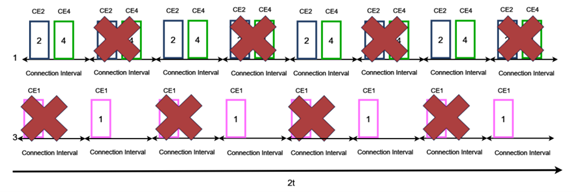
\includegraphics[width = 0.8\textwidth]{image/傳輸機制的節點時序示例.png}
    \caption{傳輸機制的節點時序示例\cite{112TIT00392032}}
    \label{fig: 傳輸機制的節點時序示例}
\end{figure}

\section{Nordic Semiconductor nRF52840}
nRF52840 是 nRF52 系列中很先進的成員,專為應對需要協定並行處理和複雜應用挑戰的需求而設計。它提供充裕的快閃記憶體與 RAM 空間,能滿足高性能應用的需求。
nRF52840 支援多協定並行運作,包含低功耗藍牙、藍牙 Mesh 網狀網路、Thread、Zigbee、IEEE 802.15.4、ANT 及 2.4 GHz 專有協定,讓其在多種應用場景中均表現出色。

此 SoC 採用 32 位元 ARM® Cortex™-M4 處理器,具備浮點運算單元,主頻達 64 MHz。內建 NFC-A 標籤,可簡化裝置配對或用於支付應用。此外,晶片搭載 ARM TrustZone® CryptoCell 安全加密單元,能在 CPU 之外高效處理加密演算法,提供強大的安全性。

nRF52840 也整合多種數位周邊和介面,包括高速 SPI 與 QSPI,能連接外部快閃記憶體與顯示裝置;PDM 與 I2S 接口用於連接數位麥克風與音訊設備。此外,內建全速 USB 控制器,支援資料傳輸功能,亦可作為電池充電的電源來源。

透過先進的片上自適應電源管理系統,nRF52840 實現了極低功耗,適合各類高效能且低能耗的應用需求,所以選用Nordic Semiconductor的nRF52840-DK開發板\cite{nordic2023softdevices}作為本次的硬體設備,如圖\ref{fig: nRF52840-DK開發板}所示
。

\begin{figure}[H]
    \centering
    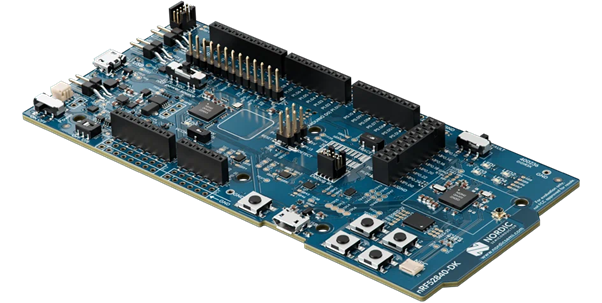
\includegraphics[width = 0.8\textwidth]{image/nRF52840-DK開發板.png}
    \caption{nRF52840-DK開發板\cite{nordic2023softdevices}}
    \label{fig: nRF52840-DK開發板}
\end{figure}

\section{FruityMesh開發平台介紹}
FruityMesh \cite{fruitymesh2023} 專為 BLE Mesh Network設計的開源通訊協定框架。該平台主要針對 Nordic Semiconductor 所推出之 nRF52 系列晶片(例如 nRF52832、nRF52840)進行最佳化,提供節點之間低功耗、穩定且具擴展性的無線通訊能力,廣泛應用於物聯網(IoT)場景。

FruityMesh 架構底層結合 Nordic SoftDevice 的藍牙堆疊,搭配即時任務管理與連線資源控管模組,能夠有效分配 Mesh 內部的連線插槽(Connection Slots)與角色權限。此外,其內建的 Clustering 與 Routing 機制可支援點對點封包傳遞與多跳路由(Multi-hop),達成資料有效分散與收斂的設計目標。

本研究即基於 FruityMesh 為開發基礎,進一步修改其拓樸建立、排程控制、連線優化與自我修復(Self-Healing)機制,以因應實際多節點部署中所可能遭遇的延遲、壅塞與節點斷線等問題。

\subsection{Nordic SoftDevice}
SoftDevice 是由 Nordic Semiconductor \cite{nordic2023softdevices} 提供的一組 預編譯、經過認證 的無線通訊定堆疊 (Protocol Stack),專為nRF系列(如nRF52840、nRF52832)等Bluetooth Low Energy(BLE)與ANT無線晶片設計。SoftDevice主要負責BLE 通訊協定的完整實作,並且以軟體庫的形式提供,方便嵌入式開發者在不需理解底層協定的情況下進行無線應用開發。

\subsection{FruityMesh Cluster}
在 FruityMesh \cite{fruitymesh2023} 架構中,Cluster(叢集)機制扮演了關鍵的角色。該機制允許網路中的節點根據功能或地理位置進行分組,以降低整體網路中不必要的廣播與封包重傳,進而提升通訊效率與穩定性。每個 Cluster 可被視為一個子網,其內部節點之間擁有穩定的連線關係,並可視需求與其他 Cluster 建立通訊橋接,使整體網路具備良好的可擴展性與模組化管理能力。

當一個節點首次啟動時,會主動進入 High Discovery 狀態,並開始廣播 JOIN 封包以尋找可連接的節點。隨著時間推進,鄰近節點會逐步聚合形成數個 Cluster,並根據連線策略逐步合併成為一個完整的網狀結構。在 FruityMesh 的預設演算法中,節點在選擇連線對象時會優先考量 Cluster 的節點數量,傾向加入節點較多的 Cluster。因此,整體網路會自然形成「大 Cluster 併吞小 Cluster」的現象,最終形成一個包含所有節點的 Spanning Tree 拓樸結構。

\subsection{FruityMesh Self-Healing}
為強化網路穩定性,FruityMesh \cite{fruitymesh2023} 同時設計了 Self-Healing(自我修復)機制。當網路中某個節點因掉電、移動或干擾等原因導致斷線,系統會自動啟動恢復流程。具體而言,斷線的節點會立即廣播連線請求封包至其通訊範圍內的所有鄰近節點。一旦鄰近節點接收到該封包,便會與之進行連線協商程序,使該孤立節點得以重新加入原有網路拓樸中。

此機制基於 FruityMesh 支援的多跳傳輸設計,確保即使部分節點失效,網路仍可自動尋找可行的替代路徑傳遞資料。Self-Healing 機制大幅提升了 BLE Mesh 系統在實際部署環境中的容錯性與可靠性,亦減少了人工維護與手動重連的需求,對於物聯網應用中的大規模部署具有重要意義。

\end{ZhChapter}